\documentclass[a4paper, 12pt]{article}

\def \srcdir{tex/}
\def \picdir{pic/}

\input{\srcdir properties}
\input{\srcdir macros}

\title{
  Лабораторная работа \textnumero \input{\srcdir index}\\
  \textbf{\textquote{\input{\srcdir name}\unskip}}
}
\author{\input{\srcdir author}}
\date{\input{\srcdir date}}

\begin{document}

\maketitle\thispagestyle{fancy}

\subsection*{Цель работы}
Измерить коэффициент теплопроводности воздуха при атмосферном\
давлении в зависимости от температуры.

\subsection*{Оборудование}
\begin{itemize}[noitemsep]
  \item Цилиндрическая колба с натянутой по оси нитью
  \item Термостат
  \item Вольтметр и амперметр (цифровые мультиметры)
  \item Эталонное сопротивление
  \item Источник постоянного напряжения
  \item Магазин сопротивлений
\end{itemize}

\subsection*{{Ход работы}}
\subsubsection*{\Rnum{1}. Теоретическое введение}

Рассмотрим стационарную теплопроводность в цилиндрической геометрии (см. \textbf{рис. \ref{fig:1}}).\
Пусть тонкая нить радиусом $r_1$ и длиной $L$ помещена на оси цилиндра радиусом $r_0$.\
Температура стенок цилиндра $T_0$ поддерживается постоянной. Пусть в нити выделяется\
некоторая тепловая мощность $Q$ [Вт]. Если цилиндр длинный $(L \gg r_0)$, можно пренебречь\
теплоотводом через его торцы. Тогда все параметры газа можно считать зависящими только\
от расстояния до оси системы $r$, а поток тепла $\vec{q}$ направленным строго радиально.\
Закон Фурье для нашей системы имеет вид
\begin{equation}
  q = -\kappa \frac{\mathrm{d}^{} T}{\mathrm{d} r^{}}.
\end{equation}
В стационарном состоянии полный поток тепла через любую цилиндрическую поверхность\
радиуса $r$ площадью $S = 2 \pi rL$ должен быть одинаков и равен $Q = qS$:
\begin{equation} \label{eq:2}
  Q = -2 \pi r L \cdot \kappa \frac{\mathrm{d}^{} T}{\mathrm{d} r^{}} = \text{const}.
\end{equation}
\begin{wrapfigure}{r}[0mm]{35mm}
  \caption{Геометрия задачи}\label{fig:1}
  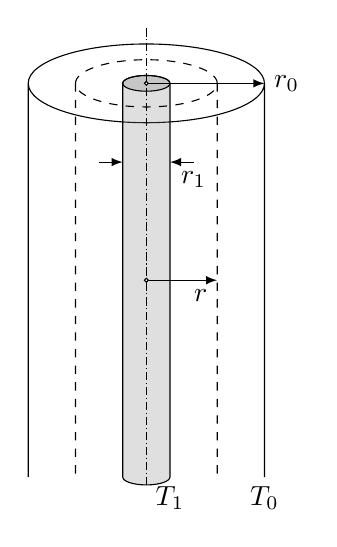
\begin{tikzpicture}[>=latex]
    \coordinate (A) at (10mm,50mm);
    \coordinate (B) at (40mm,50mm);
    \coordinate (C) at (40mm,0);
    \coordinate (D) at (10mm,0);
    \draw
    (A) arc (180:-360:15mm and 5mm)
    (A) -- (D)
    (B) -- (C);
    \node[below] at (C) {$T_0$};

    \coordinate (a) at (22mm,50mm);
    \coordinate (b) at (28mm,50mm);
    \coordinate (c) at (28mm,0);
    \coordinate (d) at (22mm,0);
    \draw [fill=gray, fill opacity=0.25]
    (a) -- (d)
    arc (180:360:3mm and 1mm)
    (c) -- (b)
    arc (0:180:3mm and 1mm);
    \draw [fill=gray, fill opacity=0.25]
    (25mm,50mm) circle (3mm and 1mm);
    \node[below] at (c) {$T_1$};

    \coordinate (a') at (16mm,50mm);
    \coordinate (b') at (34mm,50mm);
    \coordinate (c') at (34mm,0);
    \coordinate (d') at (16mm,0);
    \draw [dashed]
    (a') arc (180:-360:9mm and 3mm)
    (a') -- (d')
    (b') -- (c');

    \draw [densely dashdotted] (25mm,57mm) -- (25mm,-1mm);
    \draw
    (25mm,50mm) node [anchor=center, circle, draw, solid, inner sep=.5pt, fill=white] {}
    edge [->] node [pos=1, right] {$r_0$} +(15mm,0)
    (19mm,40mm) edge [->] +(3mm,0)
    (31mm,40mm) edge [->] node [pos=0, below] {$r_1$} +(-3mm,0)
    (25mm,25mm) node [anchor=center, circle, draw, solid, inner sep=.5pt, fill=white] {}
    edge [->] node [pos=1, below left] {$r$} +(9mm,0);
  \end{tikzpicture}
\end{wrapfigure}
Если перепад температуры $\Delta T = T_1 - T_0$ между нитью и стенками цилиндра мал\
$(\Delta T \ll T_0)$, то в (4) можно пренебречь изменением теплопроводности от температуры\
в пределах системы, положив $\kappa \approx \kappa(T_0)$. Тогда разделяя переменные в \eqref{eq:2} и\
интегрируя от радиуса нити до радиуса колбы, получим
\begin{equation}
Q = \frac{2 \pi L}{\ln{\sfrac{r_0}{r_1}}}\kappa \Delta T.
\end{equation}

\subsubsection*{\Rnum{2}. Описание установки и методики измерений}
Схема установки приведена на \textbf{рис. \ref{fig:2}}. На оси полой цилиндрической\
трубки с внутренним диаметром $2r_0 \approx 2$ см размещена металлическая нить диаметром\
$2r_1 \approx 0.05$ мм и длиной $L \approx 40$ см (материал нити и точные геометрические размеры\
указаны в техническом описании установки). Полость трубки заполнена воздухом (полость\
через небольшое отверстие сообщается с атмосферой). Стенки трубки помещены в кожух,\
через которых пропускается вода из термостата, так что их температура $t_0$ поддерживается\
постоянной. Для предотвращения конвекции трубка расположена вертикально. Металлическая\
нить служит как источником тепла, так и датчиком температуры (термометром сопротивления).\
По пропускаемому через нить постоянному току $I$ и напряжению $U$ на ней вычисляется\
мощность нагрева по закону Джоуля–Ленца:
\begin{equation}
  Q = UI,
\end{equation}
и сопротивление нити по закону Ома:
\begin{equation}
  R = \frac{U}{I}.
\end{equation}

\begin{wrapfigure}{L}[0mm]{50mm}
  \caption{Схема установки}\label{fig:2}
  \begin{circuitikz}[>=latex]
    \draw [fill=gray, fill opacity=0.25]
    (0,0) -- ++(-2mm,0)
    -- ++(0,-3mm)
    -- ++(-8mm,0)
    -- ++(0,-3mm)
    -- ++(8mm,0)
    -- ++(0,-38mm)
    -- ++(-8mm,0)
    -- ++(0,-3mm)
    -- ++(8mm,0)
    -- ++(0,-3mm)
    -- ++(2mm,0)
    -- ++(0,50mm)
    (8mm,0) -- ++(0,-50mm)
    -- ++(2mm,0)
    -- ++(0,50mm)
    -- ++(-2mm,0);

    \draw [fill=gray, fill opacity=0.5]
    (0,0) -- ++(8mm,0)
    -- ++(0,-2mm)
    -- ++(-8mm,0)
    -- ++(0,2mm)
    (0,-50mm) -- ++(8mm,0)
    -- ++(0,2mm)
    -- ++(-8mm,0)
    -- ++(0,-2mm);

    \draw
    (12mm,2mm) node[right] {\footnotesize{к цепи}}
    node [anchor=center, circle, draw, solid, inner sep=.5pt, fill=white] {}
    -- ++(-8mm,0)
    -- ++(0mm,-4mm)
    -- ++(1pt,-1pt)
    -- ++(-2pt,-1pt)
    -- ++(2pt,-1pt)
    -- ++(-2pt,-1pt)
    -- ++(2pt,-1pt)
    -- ++(-1pt,-1pt)
    node [anchor=center, circle, draw, solid, inner sep=.5pt, fill=black] {}
    (12mm,-52mm) node [anchor=center, circle, draw, solid, inner sep=.5pt, fill=white] {}
    -- ++(-8mm,0)
    -- ++(0mm,5mm)
    node [anchor=center, circle, draw, solid, inner sep=.5pt, fill=black] {};

    \draw [line width=0.4mm]
    (4mm,-4mm) -- ++(0,-43mm);

    \draw [densely dotted]
    (4mm,-4mm) -- (16mm,-4mm)
    (4mm,-47mm) -- (16mm,-47mm);

    \draw [<->] (16mm,-4mm) -- (16mm,-47mm);
    \draw (16mm,-25mm) node [fill=white] {$L$};

    \draw [->] (-10.5mm,-4.5mm) -- ++(-4mm,0)
    node [above=1mm] {\footnotesize{к термостату}};

    \draw [<-] (-10.5mm,-45.5mm) -- ++(-4mm,0)
    node [below=1.5mm] {\footnotesize{от термостата}};

    \draw [->] (4.2mm,-40mm) -- ++(3.8mm,0)
    node [left=1.7mm,below] {\footnotesize{$r_0$}};

    \draw [->] (8mm,-35mm) -- ++(-3.8mm,0);
    \draw [->] (0mm,-35mm)
    -- ++(3.8mm,0)
    node [left=2.9mm, below=1mm, fill=white, inner sep=0.9pt] {\footnotesize{$2r_1$}};
    
    \draw [densely dotted]
    (4mm,-30mm) -- ++(-10mm,5mm)
    node [left] {\footnotesize{нить}};
  \end{circuitikz}
\end{wrapfigure}

Сопротивление нити является однозначной функцией её температуры $R(t)$. Эта зависимость\
может быть измерена с помощью термостата по экстраполяции мощности нагрева к нулю\
$Q \rightarrow 0$, когда температура нити и стенок совпадают $t_1 \approx t_0$. Альтернативно, если\
материал нити известен, зависимость его удельного сопротивления от температуры может\
найдена по справочным данным. Для большинства металлов изменение сопротивления из-за\
нагрева невелико: при изменении температуры на $\Delta t = 1\ ^\circ C$ относительное изменение\
сопротивления нити $\frac{\Delta R}{R}$ может составлять приблизительно от $0.2\%$ до $0.6\%$\
(в зависимости от её материала). Следовательно, измерение $R$ важно провести с высокой\
точностью. Желательно, чтобы методика измерений и чувствительность приборов обеспечивали\
измерение тока и напряжения с относительной погрешностью, не превышающей $0.1\%$\
(т.е. необходимо уверенно измерять 4–5 значащих цифр, что вполне реально при использовании\
современных цифровых мультиметров).

На \textbf{рис. \ref{fig:3}} приведена электрическая схема установки. Для измерения\
напряжения и тока используется два мультиметра, работающие в режимах вольтметра и\
амперметра соответственно. Подключение к нити $R_н$ осуществляется по четырёхпроводной\
схеме. По двум проводам (токовая пара $I_+$ и $I_-$) через сопротивление пропускается\
измерительный ток, а два других (потенциальная пара $U_+$ и $U_-$) используются для\
параллельного подключения вольтметра. Сопротивление $R_э$ используется в качестве\
балластного для предотвращения перегорания нити. Заметим, что при такой схеме\
внутреннее сопротивление приборов и сопротивление подводящих проводов практически\
не влияет на измерения: сопротивление амперметра не влияет на результат вовсе, а\
сопротивление вольтметра составляет обычно $1–100$ МОм, что при $R_н \approx 10$ Ом вносит\
относительную ошибку не более $10^{-5}$. Ток в цепи в обеих схемах регулируется с\
помощью магазина сопротивлений $R_м$, включённого последовательно с источником напряжения.
\begin{wrapfigure}{r}[0mm]{60mm}
  \caption{Электрическая схема для измерения нагрузочной кривой}\label{fig:3}
  \begin{circuitikz}[>=latex, american]
    \draw (0,0)
    to [battery2, invert, l_={$\mathscr{E}$}] ++(10mm,0)
    to [tgeneric, l={$R_м$}] ++(20mm,0)
    node [anchor=center, circle, draw, solid, inner sep=.5pt, fill=black] {}
    node [right=2mm, above] {\footnotesize{$I_+\ U_+$}}
    to [generic, l_={$R_н$}] ++(0,-40mm)
    node [anchor=center, circle, draw, solid, inner sep=.5pt, fill=black] {}
    node [right=2mm, below] {\footnotesize{$I_-\ U_-$}}
    to [generic, l_={$R_э$}] ++(-30mm,0)
    to [rmeter, t=A, i=$I$] (0,0)
    (30mm,0) -- ++(15mm,0)
    to [rmeter, t=V, v^=$U$] ++(0,-40mm)
    -- ++(-15mm,0);
  \end{circuitikz}
\end{wrapfigure}
В исследуемом интервале температур (20---80 $^\circ C$) зависимость сопротивления от\
температуры можно с хорошей точностью аппроксимировать линейной функцией:
\begin{equation} \label{eq:6}
  R(t) = R_{273} \cdot (1 + \alpha t),
\end{equation}
где $t$ --- температура в $[^\circ C]$, $R_{273}$ --- сопротивление нити при температуре $0\ ^\circ C$ и
\begin{equation}
  \alpha = \frac{1}{R_{273}} \frac{\mathrm{d}^{} R}{\mathrm{d} T^{}}
\end{equation}
--- температурный коэффициент сопротивления материала. Измерение зависимости \eqref{eq:6}\
по данным для $Q \rightarrow 0$ позволит затем определять температуру нити $t$ по значению\
её сопротивления $R$ при произвольной мощности нагрева.

\subsubsection*{\Rnum{3}. Пиво \textquote{Невское}}
\lipsum[6-6]

\subsection*{{Вывод}}

\lipsum[7-7]

\end{document}


